\newpage
\section{Details on the Müller method}

\subsection{The root-finding algorithm}
equations, iterative scheme etc. 

\cite{chapra2010}

\begin{equation}
    \begin{aligned}
        f(x_0)&=a(x_0-x_2)^2+b(x_0-x_2)\\
        f(x_1)&=a(x_1-x_2)^2+b(x_1-x_2)\\
        f(x_2)&=a(x_2-x_2)^2+b(x_2-x_2)
    \end{aligned}
\end{equation}

Note that we have dropped the subscript“2” from the function for conciseness. Because we have three equations, we can solve for the three unknown coefficients, $a,b$,and $c.$ Because two of the terms in Eq. (7.20) are zero, it can be immediately solved for $c=f(x_{2}).$ Thus, the coefficient $c$ is merely equal to the function value evaluated at the third guess, $x_2.$ This result can then be substituted into Eqs. (7.18) and (7.19) to yield two equations with two unknowns:

$$\begin{aligned}
    f(x_0)-f(x_2)&=a(x_0-x_2)^2+b(x_0-x_2)\\
    f(x_1)-f(x_2)&=a(x_1-x_2)^2+b(x_1-x_2)\end{aligned}$$

Algebraic manipulation can then be used to solve for the remaining coefficients, $a$ and $b.$
One way to do this involves defining a number of differences,

$$\begin{aligned}h_0&=x_1-x_0&h_1&=x_2-x_1\\\delta_0&=\frac{f(x_1)-f(x_0)}{x_1-x_0}&\delta_1&=\frac{f(x_2)-f(x_1)}{x_2-x_1}\end{aligned}$$


These can be substituted into Eqs.(7.21) and (7.22) to give
$$\begin{aligned}(h_0+h_1)b-(h_0+h_1)^2a&=h_0\delta_0+h_1\delta_1\\h_1\quad b-\quad h_1^2\quad a&=\quad h_1\delta_1\end{aligned}$$

which can be solved for $a$ and $b.$The results can be summarized as
(7.24)
$$\begin{aligned}&a=\frac{\delta_{1}-\delta_{0}}{h_{1}+h_{0}}\\&b=ah_{1}+\delta_{1}\\&c=f(x_{2})\end{aligned}$$
(7.25) (7.26)
To find the root, we apply the quadratic formula to Eq. (7.17). However, because of potential round-off error, rather than using the conventional form, we use the alternative formulation [Eq.(3.13)] to yield
$$x_3-x_2=\frac{-2c}{b\pm\sqrt{b^2-4ac}}$$

or isolating the unknown $x_3$ on the left side of the equal sign,

$$x_3=x_2+\frac{-2c}{b\pm\sqrt{b^2-4ac}}$$


Note that the use of the quadratic formula means that both real and complex roots can be
located. This is a major benefit of the method.
In addition, Eq. $(7.27a)$ provides a neat means to determine the approximate error. Because the left side represents the difference between the present $(x_3)$ and the previous $(x_2)$ root estimate, the error can be calculated as

$$\varepsilon_a=\left|\frac{x_3-x_2}{x_3}\right|100\%$$
\begin{figure}[h!]
    \centering
    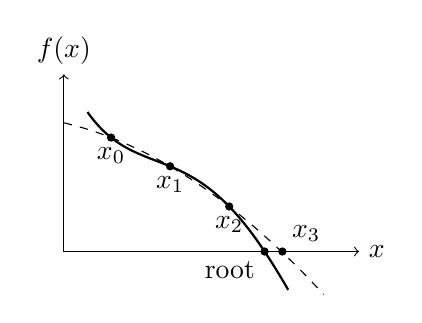
\begin{tikzpicture}[scale=1.5,domain=-.5:1.2]
        \draw[thick] plot[samples=100] (
            \x, {0.3*(\x)^4 - 0.9*(\x)^3 + 0.2*(\x)^2 - 0.4*(\x) + 0.8});
        
        \pgfmathsetmacro{\xzero}{-.3}
        \pgfmathsetmacro{\yzero}{0.3*(\xzero)^4 - 0.9*(\xzero)^3 + 0.2*(\xzero)^2 - 0.4*(\xzero) + 0.8}
        \pgfmathsetmacro{\xone}{0.2}
        \pgfmathsetmacro{\yone}{0.3*(\xone)^4 - 0.9*(\xone)^3 + 0.2*(\xone)^2 - 0.4*(\xone) + 0.8}
        \pgfmathsetmacro{\xtwo}{.7}
        \pgfmathsetmacro{\ytwo}{0.3*(\xtwo)^4 - 0.9*(\xtwo)^3 + 0.2*(\xtwo)^2 - 0.4*(\xtwo) + 0.8}
        \pgfmathsetmacro{\xthree}{1}
        \pgfmathsetmacro{\ythree}{0}
        
        % Draw points
        \fill (\xzero,\yzero) circle (1pt) node[below] {$x_0$};
        \fill (\xone,\yone) circle (1pt) node[below] {$x_1$};
        \fill (\xtwo,\ytwo) circle (1pt) node[below] {$x_2$};
        
        % Compute coefficients for the parabolic interpolation
        \pgfmathsetmacro{\a}{(\yzero/((\xzero-\xone)*(\xzero-\xtwo))) + (\yone/((\xone-\xzero)*(\xone-\xtwo))) + (\ytwo/((\xtwo-\xzero)*(\xtwo-\xone)))}
        \pgfmathsetmacro{\b}{(\yzero*(\xone+\xtwo)/((\xzero-\xone)*(\xzero-\xtwo))) + (\yone*(\xzero+\xtwo)/((\xone-\xzero)*(\xone-\xtwo))) + (\ytwo*(\xzero+\xone)/((\xtwo-\xzero)*(\xtwo-\xone)))}
        \pgfmathsetmacro{\c}{(\yzero*\xone*\xtwo/((\xzero-\xone)*(\xzero-\xtwo))) + (\yone*\xzero*\xtwo/((\xone-\xzero)*(\xone-\xtwo))) + (\ytwo*\xzero*\xone/((\xtwo-\xzero)*(\xtwo-\xone)))}
        
        \draw[dashed] plot[samples=50,domain=-.7:1.5] (
            \x, {\a*(\x)^2 - \b*\x + \c}
        );
        \fill (\xthree,\ythree) circle (1pt) node[below left] {root};
        \fill (1.15,0) circle (1pt) node[above right] {$x_3$};
        % Axes
        \draw[->] (-.7,0) -- (1.8,0) node[right] {$x$};
        \draw[->] (-.7,0) -- (-.7,1.5) node[above] {$f(x)$};
    \end{tikzpicture}       
    \caption{iteration muller}
\end{figure}

\subsection{A complete routine for the automated solving of dispersion relations}
\begin{figure}[h!]
    \centering
    \tikzstyle{case} = [rectangle, rounded corners, text width=3.5cm, minimum height=1cm,text centered, draw=black]
    \tikzstyle{arrow} = [thick,->]
    \tikzstyle{arrowlabels} = [midway, fill=white, text width=3cm, rounded corners, text centered, inner sep=5pt]
    \begin{tikzpicture}[node distance=3cm]
        \node (params) [text width=4cm] {$\bullet$ Parameters};
        \node (func) [text width=4cm, below=.1cm of params] {$\bullet$ function determinant};
        \node (freq) [text width=4cm, below=.1cm of func] {$\bullet$ Given frequency $f_i$};
        \node[case,fit={(params) (func) (freq)}, inner sep=10pt]  (init) {};
        % \node (init) [case] {parameter \\function};
        \node (map) [case, below=1.5cm of init] {Determinant mapping};
        \node (rootfind) [case, below of=map] {Müller method for each guess};
        \node (modeshape) [case, below of=rootfind] {Mode shapes};
        \node (store) [case, left= 1cm of modeshape]{Output and store data};
        \draw [arrow] (init) -- (map)node[arrowlabels] {{\color{accent} if no guesses}};
        \draw [arrow] (init) -- ++ (-4, 0)  -- ++ (0, -6.4) node[arrowlabels] {{\color{accent} if guesses}}-- (rootfind) ;
        \draw [arrow] (map) -- (rootfind)node[arrowlabels] {local minima used as guesses};
        \draw [arrow] (rootfind) -- (modeshape)node[arrowlabels, text width=.8cm] (roots) {roots};
        \draw [arrow] (roots) -- ++ (3.7,0) -- node[arrowlabels] {{\color{accent} if not enough found roots} (only once)} ++ (0,4.5) -- (map);
        \draw [arrow] (roots) -- ++ (6,0) -- node[arrowlabels] {{\color{accent} if enough found roots} use as guesses and go to next frequency $f_{i+1}$} ++ (0,7.9) -- (init);
        \draw[arrow] (roots) -- ++ (-4.78, 0) -- ++ (0, -.8) -- (store);
        \draw[arrow] (modeshape) -- (store);
    \end{tikzpicture}
    \caption{Description of the routine}
\end{figure}